\documentclass[../main.tex]{subfiles}

\begin{document}
    
\chapter{Candidate Universe Ranking}
    
Following the successful derivation of an objective sector classification heuristic (addressing RG-1), the next step is to derive a methodology to rank our sectors against each other, to isolate the optimal sector/sectors, without imposing any subjective criteria on the selection. Thus, this section begins the discussion of addressing the second research goal, RG-2 (see Section~\ref{research_goals:specific_research_goals}):

\begin{table}[h!]
    \centering
    \begin{tabular}{| c | c |}
        \hline
        &  \\
        RG-2 & Rank candidate sector universes against each other using entirely objective criteria. \\
        & \\
        \hline
    \end{tabular}
    \caption{Specific project research goal RG-2.}
    \label{table:candidate_universe_ranking:research_goal}
\end{table}

\section{Sample Learned Sector Universe}

\begin{wrapfigure}[18]{r}{0.5\textwidth}
    \centering
    \vspace{\wrapfigadjustment}
    \fbox{
    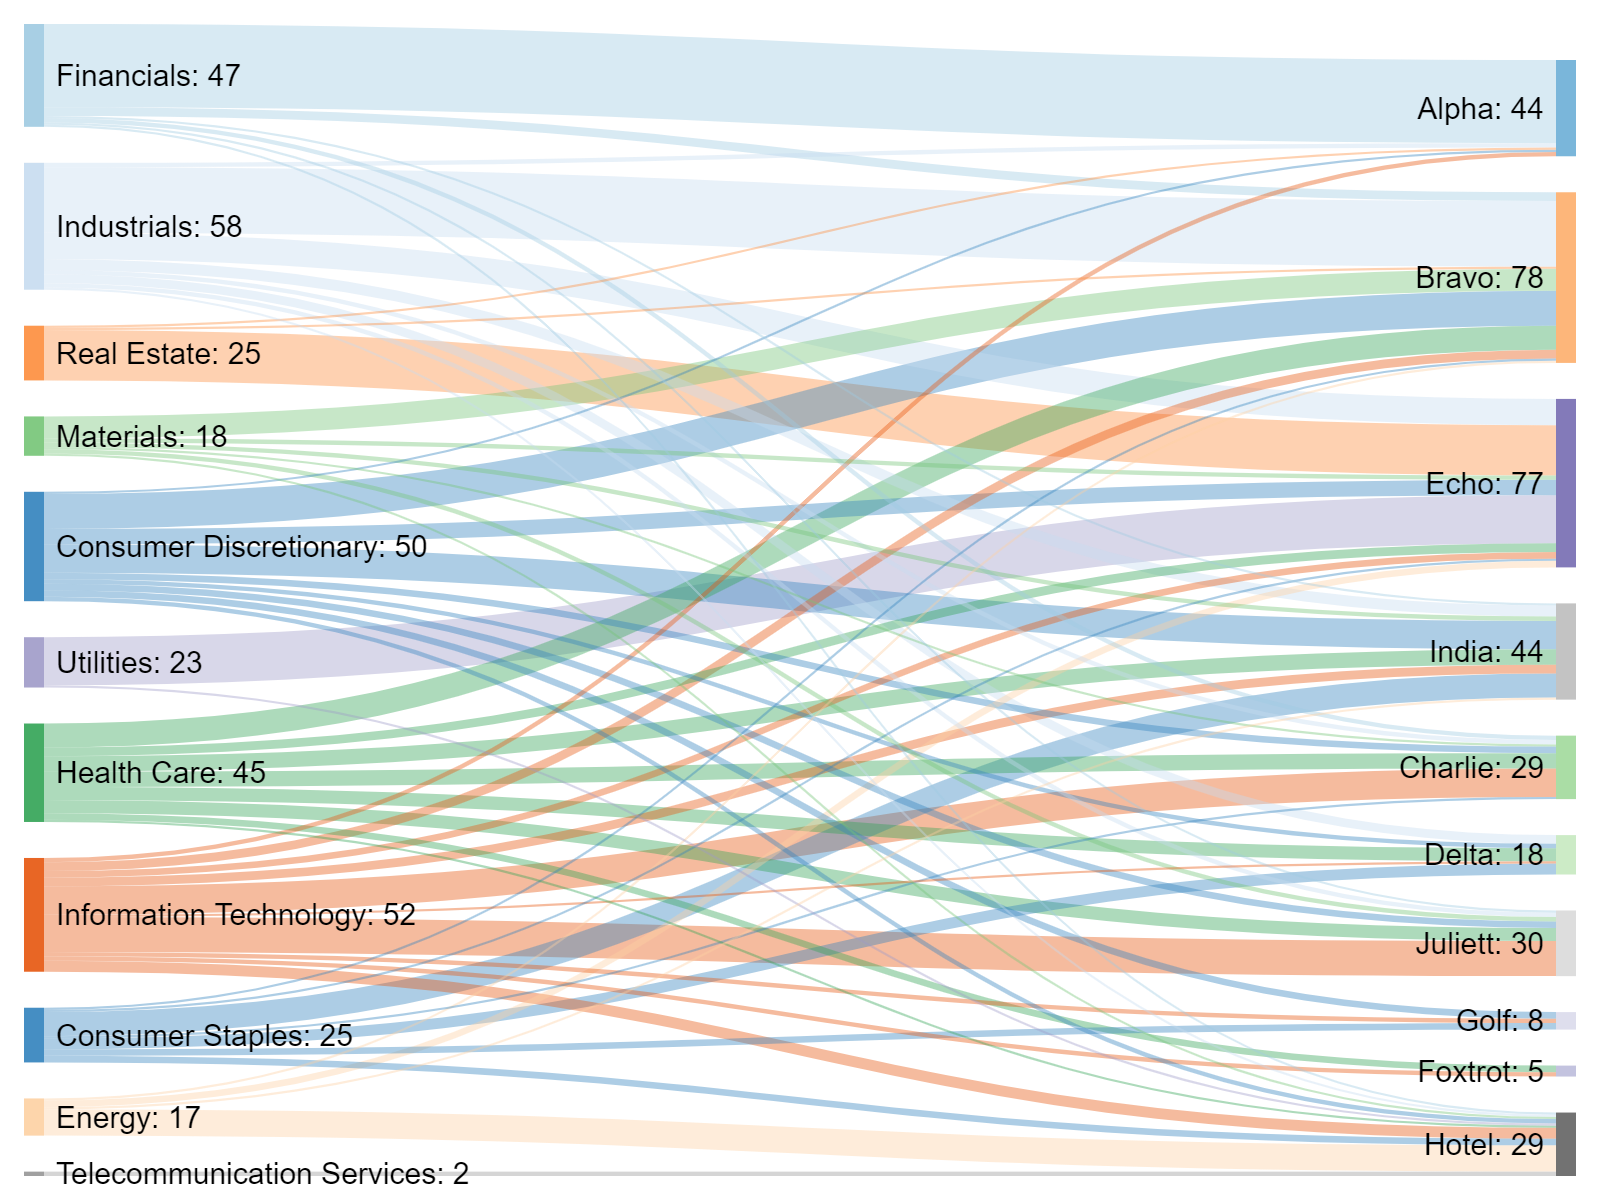
\includegraphics[width=0.48\textwidth]{images/sample_ls_universe.png}
    }
    \caption{Sample learned sector universe - Ward Linkage; 2010 Data; 10 Sectors.}
    \label{fig:candidate_universe_ranking:sample_ls_universe}
\end{wrapfigure}

To best motivate the approach we decided to use when comparing and ranking candidate sector universes, it is worthwhile to discuss an example.

Figure~\ref{fig:candidate_universe_ranking:sample_ls_universe} is a Sankey Diagram, representing the new learned sector assignments of various corporations from our search space by means of comparison to the benchmark. The left-hand side of the diagram represents the original benchmark sectors, and their constituent assets, while the right hand side represents the new learned sector assignment of the same assets.

As evidenced by the diagram, there appears to be significant transitory behavior of corporations across sectors when comparing the benchmark sectors to the learned sectors. Additionally, there also appears to be a significant amount of mixing between the sectors, with very few sectors appearing to be preserved between the sector universes. In the example, the only sector that can be considered remotely similar to a benchmark sector would be learned sector \textit{Alpha} to benchmark sector \textit{Financials}.

Other sectors however, appear largely broken up and dispersed when comparing their benchmark sector to the new learned sector univese. Particularly noticable examples of this include the benchmark sectors \textit{Health Care}, \textit{Information Technology}, and \textit{Consumer Discretionary}. Due to the fundamentals-driven nature of our classification heuristic, this result is not entirely surprising; the benchmark sectors that appear to have the most dispersion in the learned sector universe are ones which are increasingly integral to regular business, regardless of sector; particularly \textit{Information Technology}.

As illustrated in this section with a single example, there is extremely little congruity between the benchmark sector classification and the learned sector classification. This pattern can be observed across a larger set of learned sector universes in Figure~\ref{fig:hierarchical_clustering_model:partial_search_space}, a partial visualization of the learned sector search space.

Due to this fact, is would be extremely difficult to perform a sector-by-sector analysis across sector universes as a means for comparison. There is obvious difficulty in matching sectors across universes (as illustrated by the example in Figure~\ref{fig:candidate_universe_ranking:sample_ls_universe}) without introducing significant bias to the comparison metric. Furthermore, there is an additional issue presented by the fact that the number of sectors in two given candidate learned sector universes may not be identical (let alone the number of constituent corporations in a given sector), thus completely prohibiting a sector-by-sector analysis.

To combat this issue, we decided to evaluate the sector universes as a whole, and then analyze universe-level metrics to rank the candidate learned sectors. To this end, we developed \textit{reIndexer}, which is discussed at length in the following section.

\section{reIndexer}

\begin{wrapfigure}[18]{r}{0.4\textwidth}
    \centering
    \vspace{\wrapfigadjustment}
    \fbox{
    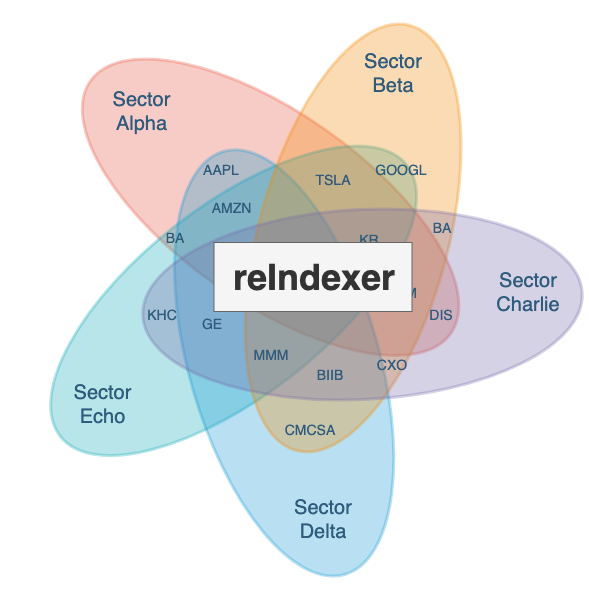
\includegraphics[width=0.38\textwidth]{images/reIndexer_logo.png}
    }
    \caption{The \textit{reIndexer} research tool.}
    \label{fig:candidate_universe_ranking:reindexer_logo}
\end{wrapfigure}

\textit{reIndexer}\citeFormat{\cite{Weerawarana2019ReIndexerUniverses}} is an open-source research tool for backtest-driven evaluation of different sector universes, using a system of Synthetic ETFs (hereafter \textit{SETF}), and efficient portfolios of those SETFs. reIndexer was designed and implemented to solve the problem discussed in the previous section; namely, the fact that we cannot perform a sector-by-sector comparison, and thus must compare learned sectors at the universe-level.

Built on Quantopian's \textit{Zipline Pythonic Algorithmic Trading Library}\citeFormat{\cite{QuantopianInc.2019ZiplineLibrary}}, reIndexer is fully API-compatible with Quantopian's suite of analytics tools, including \textit{Alphalens}\citeFormat{\cite{QuantopianInc.2019AlphalensFactors}} and \textit{Pyfolio}\citeFormat{\cite{QuantopianInc.2019PyfolioPython}}. While these libraries are not directly used in this project, the modular design of reIndexer make it an extremely powerful platform that is highly extensible in scope and functionality.

reIndexer was designed under the the hypothesis that the universe-level statistics of a given sectorization scheme would provide a superior metric for comparison across sector universes, compared to a sector-by-sector analysis. To this end - at a very high level - it provides a level of abstraction between single-asset trades, and constructed SETFs (whose composition is provided by the user), to simulate and record the performance of a portfolio of these SETFs over a predefined backtesting window.

\subsection{Synthetic ETF Formulation}

As the assets prescribed by the classification heuristic are not traded in the real market, it is not possible to get historical ETF prices directly from Zipline's engine. reIndexer works around this fact by implementing a layer between the portfolio optimization, and the assets, maintaining a hypothetical SETF. To compute efficient portfolios, and to treat the SETFs as unique assets from the point of view of the portfolio optimization engine, all that is necessary is a historical chain of prices for a given asset, over a specified lookback period.

To this end, reIndexer currently implements a price-weighted synthetic ETF. The pythonic implementation of this ETF is based on a highly flexible and reproducible tempalte, ensuring that different types of ETFs (market-weighted, etc.) can be easily implemented and used with reIndexer. For this project, price-weighted SETFs were used due to the fact that Zipline does not have historical market capitalization data for certain firms in its asset universe.

The mathematical formulation of the price-weighted SETF is outlined below:

\begin{gather*}
    \text{Let $\boldsymbol{S}_\alpha$} = \text{Sample sector $\alpha$} \\
    \text{Let $\boldsymbol{P}_\alpha$} = \text{Prices of assets in $\boldsymbol{S}_\alpha$} \\
    \text{Let $\boldsymbol{w}_\alpha$} = \text{Weights of assets in $\boldsymbol{S}_\alpha$} \\
    \\
    \Rightarrow \boldsymbol{w}_\alpha = \left[ \frac{P_i}{\sum \boldsymbol{P}_\alpha} \, \forall \, P_i \in \boldsymbol{P}_\alpha \right]^\intercal
\end{gather*}

This process of recomputing the weights of the constituent assets in a SETF is referred to as \textbf{SETF Restructuring}.

Suppose that this SETF restructuring process occurs at every time step $\{ r_t, r_{t+1}, \ldots, r_{t+n} \}$.

Additionally, let there be additional time steps in-between the restructuring process times, $\{ r_{t + \delta t}, r_{t + 2\delta t}, \ldots, r_{t + m \delta t} \}$, such that {${r_t < \{ r_{t + \delta t}, \ldots, r_{t + m\delta t} \} \leq r_{t + 1}}$}.

At each of these intermediate timesteps, the price-weighted SETF will have a price equal to the dot product of the sector asset weights computed at the immediately preceding SETF restructuring time $r_{t}$, $\boldsymbol{w}_{\alpha,r_t}$ and the prices of the constituent assets at the intermediate timestep, $\boldsymbol{P}_{\alpha,r_{t+m\delta t}}$.

\begin{gather*}
    \text{Let $\Pi_{\alpha,\tau}$} = \text{Price of sector SETF $\alpha$ at time $\tau$} \\
    \\
    \Rightarrow \Pi_{\alpha,\tau_i} = \boldsymbol{w}_{\alpha, r_t} \cdot \boldsymbol{P}_{\alpha,\tau_i} \, \forall \, \tau_i \in \{ r_{t + \delta t}, r_{t + 2\delta t}, \ldots, r_{t + m \delta t} \}
\end{gather*}

reIndexer provides an extremely flexible interface to specify SETF restructuring trigger times, $\{ r_t, r_{t+1}, \ldots, r_{t+n} \}$. The restructure can be triggered on any specific day of any specific week of the month (eg: third Friday of each month), or simply the first trading day of each month. Additionally, it also handles intelligent rebalancing rollovers, in the event that the specified rebalancing date trigger is a holiday with respect to the configured trading calendar.


\subsection{Efficient Portfolio Optimization}

Following the construction of the SETFs, reIndexer builds an efficient portfolio, treating each of the SETFs as distinct, unitary assets. As our goal with the project is to assess the benefit of fundamentals-driven objective sector classifications through the lens of risk diversification, reIndexer currently implements a backtest of a Global Minimum Variance Portfolio, not allowing short-sales.

However, in a similar fashion to the price-weighted SETF, the pythonic implementation of this portfolio is highly generalized in the reIndexer source code, and can be easily reconfigurable to work with myriad different portfolio configuraitons. reIndexer provides functionality to retreive a Matrix of historical SETF prices for a given lookback window, with SETF prices being correctly computed using the formulation described above.

Following this, reIndexer computes the correlation matrix of returns using the historical prices over a specific lookback period, and then performs the non-convex optimization necessary to compute SETF weights in the Global Minimum Variance Portfolio. The mathematical formulation for this process is outlined below (note that notation is preserved from the preceding section):

\begin{gather*}
    \text{Let $\Omega$} = \text{Set of sectors in the candidate universe, $\Omega_i \in \{\Omega_1, \Omega_2, \ldots, \Omega_n\}$} \\
    \text{Let $\boldsymbol{\Pi}_{\Omega_i}$} = \text{Historical log price vector of sector SETF $\Omega_i$} \\
    \text{Let $\Sigma$} = \text{Correlation matrix of historical log-returns of SETFs } \\
    \\
    \boldsymbol{\Sigma} =
    \begin{bmatrix}
        \mathbb{E}[(\boldsymbol{\Pi}_{\Omega_1} - \mathbb{E}[\boldsymbol{\Pi}_{\Omega_1}])^2] & \mathbb{E}[(\boldsymbol{\Pi}_{\Omega_1} - \mathbb{E}[\boldsymbol{\Pi}_{\Omega_1}])(\boldsymbol{\Pi}_{\Omega_2} - \mathbb{E}[\boldsymbol{\Pi}_{\Omega_2}])] & \cdots & \mathbb{E}[(\boldsymbol{\Pi}_{\Omega_1} - \mathbb{E}[\boldsymbol{\Pi}_{\Omega_1}])(\boldsymbol{\Pi}_{\Omega_n} - \mathbb{E}[\boldsymbol{\Pi}_{\Omega_n}])] \\
        & & & \\
        \mathbb{E}[(\boldsymbol{\Pi}_{\Omega_2} - \mathbb{E}[\boldsymbol{\Pi}_{\Omega_2}])(\boldsymbol{\Pi}_{\Omega_1} - \mathbb{E}[\boldsymbol{\Pi}_{\Omega_1}])] & \mathbb{E}[(\boldsymbol{\Pi}_{\Omega_2} - \mathbb{E}[\boldsymbol{\Pi}_{\Omega_2}])^2] & \cdots & \mathbb{E}[(\boldsymbol{\Pi}_{\Omega_2} - \mathbb{E}[\boldsymbol{\Pi}_{\Omega_2}])(\boldsymbol{\Pi}_{\Omega_n} - \mathbb{E}[\boldsymbol{\Pi}_{\Omega_n}])] \\
        & & & \\
        \vdots & \vdots & \ddots & \vdots \\
        & & & \\
        \mathbb{E}[(\boldsymbol{\Pi}_{\Omega_n} - \mathbb{E}[\boldsymbol{\Pi}_{\Omega_n}])(\boldsymbol{\Pi}_{\Omega_1} - \mathbb{E}[\boldsymbol{\Pi}_{\Omega_1}])] & \mathbb{E}[(\boldsymbol{\Pi}_{\Omega_n} - \mathbb{E}[\boldsymbol{\Pi}_{\Omega_n}])(\boldsymbol{\Pi}_{\Omega_2} - \mathbb{E}[\boldsymbol{\Pi}_{\Omega_2}])] & \cdots & \mathbb{E}[(\boldsymbol{\Pi}_{\Omega_n} - \mathbb{E}[\boldsymbol{\Pi}_{\Omega_n}])^2] \\
    \end{bmatrix}
\end{gather*}


\subsection{Software Architecture Overview}

\begin{figure}[h!]
    \centering
    \fbox{
    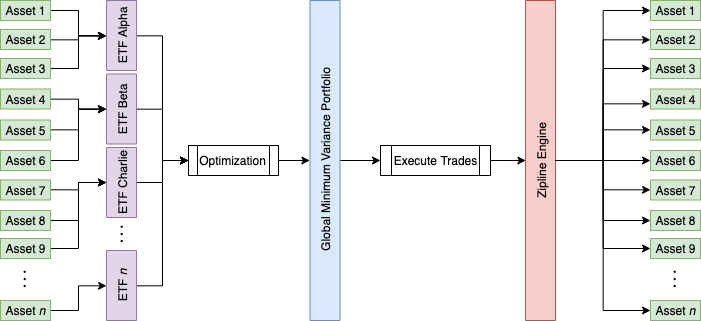
\includegraphics[width=.8\linewidth]{images/reindexer_architecture.png}
    }
    \caption{reIndexer architecture overview diagram}
    \label{fig:candidate_universe_ranking:reindexer_architecture}
\end{figure}




\end{document}